\chapter{Software}
This chapter contain the software that is used for developing and testing the autonomous landing system for uav. The software that is mainly used in the uav system is based on a open-source software toolchain developed by the Underwater System and Technology Laboratory (LSTS). The toolchain supports air and ocean vehicle systems. The different components in the toolchain is IMC, DUNE, NEPTUS and Glued, which will be presented in later in this chapter. 

The rtkgps solution in the system is calculated in the open-source software RtkLib \citep{takasu2009development}. The desceription of the program is given in section \ref{s:Rtklib}.

The low level control system in the uav is controlled by Ardupilot, which is a 
\section{LSTS toolchain}
The software that the system is based on was developed by the Underwater Systems and Technology Laboratory (LSTS), which is called the LSTS toolchain \citep{pinto2013lsts}. The toolchain was developed for support of networked heterogeneous air and ocean vehicle systems over wireless network. The toolchain contain four different modules, namely \gls{imc}, DUNE, NEPTUS and Glued.
\subsection{IMC}
\gls{imc} \citep{martins2009imc} is design to enable interconnections between systems of vehicles, sensors and human operators, which enable the pursuit of common goal by cooperatively exchange real-time information about the environment and updated objectives. The message protocol is oriented around the message, which abstracts hardware and communication heterogeneity with a provided shared set of messages that can be serialized and transferred over different means. The \gls{imc} protocol is defined in a single eXtensible Markup Language (XML) document, which simplify the definition of exiting messages and the creation of new messages. A single XML document ease communication between two node when both node use the same document for message definition. 
\subsection{Dune}
DUNE (DUNE Uniform Navigation Environment) is a runtime environment for unmanned systems on-board software written in C++. DUNE is capable to interact with sensors, payload and actuators, in addition to communication, navigation, control, manoeuvring, plan execution and vehicle supervision. The software separate operations into different task that each has there own thread of execution. DUNE apply a message bus that is responsible for forwarding \gls{imc} message from the producer to all registered receivers, which is the only way different DUNE tasks is communicating. 

A DUNE task is enabled through a configuration file, where the user can choose in which profile the task should be enabled in. The different profile configuration in DUNE allows for testing the same system used in a hardware setting with a simulator.
\subsection{Neptus}
Neptus is a Command and Control software which is used to command and monitor unmanned systems that is written in Java. Neptus is able to provide coherent visual interface to command despite the heterogeneity in the controlled system that it is interacting with.  This allow the operator to command and control unmanned system without the need to dwell into specific command and control software in the unmanned system. The main communication channel for Neptus is \gls{imc}, which makes it interoperable with DUNE or other \gls{imc}- based peer.

Neptus is able to do MRA (Mission Review and Analysis) after a mission is finished. In the MRA phase Neptus analyse the \gls{imc} logs that is collected by e.g. DUNE, such that the result from a completed mission can be presented. In addition Neptus mission review is able to create output files of the log that can be analysed in third party software like Matlab.
\subsection{Glued}
Glued is a minimal Linux operating system distribution, and design with embedded system in mind. It is platform independent, easy to configure and contain only the necessary packages to run on a embedded system. This makes GLUED a light and fast distribution, which is ideal for a on-board operating system for a unmanned system where payload size is normally limited. GLUED is configured through a single configuration file that which can be created for a specific system. A advantage with Glued is that it can be cross-compiled, which allows for compilation of software before it's transferred to the embedded computer.
\section{RTK-GPS system}
The \gls{rtk-gps} solution is calculated in the open-source program liberary RTKLib \citep{takasu2009development}.
The X8 runs the rover program rtkrcv which is connected over TCP/IP with the base station program str2str. Both programs are connected to a Ublox Lea M8T GNSS receiver. The GNSS receiver is programmed to send raw GNSS data to both programs, where the base station program str2str transmits without alteration the raw data to the rover program rtkrcv. The structure of the RTKLib software configured with a rover and base station is shown in figure \ref{figure:RTKLIB_STRUCTURE}.

The navigation system require to now the reference position of the base station in order to use the \gls{rtk-gps} solution. However the base station position is currently not part of the output message from rtkrcv. This is resolved by allowing the base station to calculate it's own position as a standalone \gls{gps}. The \gls{gps} position is transmitted to a local Dune task on the base station, where the operator can decide when the base station can be considered as fixed. When the base station is considered fixed the position is sent to the X8, where it's included in the \gls{rtk-gps} solution message.
\subsection{RTKLIB}\label{ss:Rtklib}
\acrfull{rtklib}\citep{takasu2009development} is a open source program package for standard and precise positioning with \gls{gnss} developed by T. Takasu. \gls{rtklib} can be configured to apply \gls{rtk-gps}, such that raw \gls{gnss} data is used estimate the relative position of the rover with respect to the base station in real time. Figure \ref{figure:RTKLIB_STRUCTURE} shows how \gls{rtklib} can be used in a \gls{rtk-gps} mode. The two main modules here is str2str and rtkrcv. Both will be explained more closely in the following sections. The version of \gls{rtklib} used in this thesis is \gls{rtklib}2.4.2 \citep{Rtklib242}.
\begin{figure}[H]
	\centering
		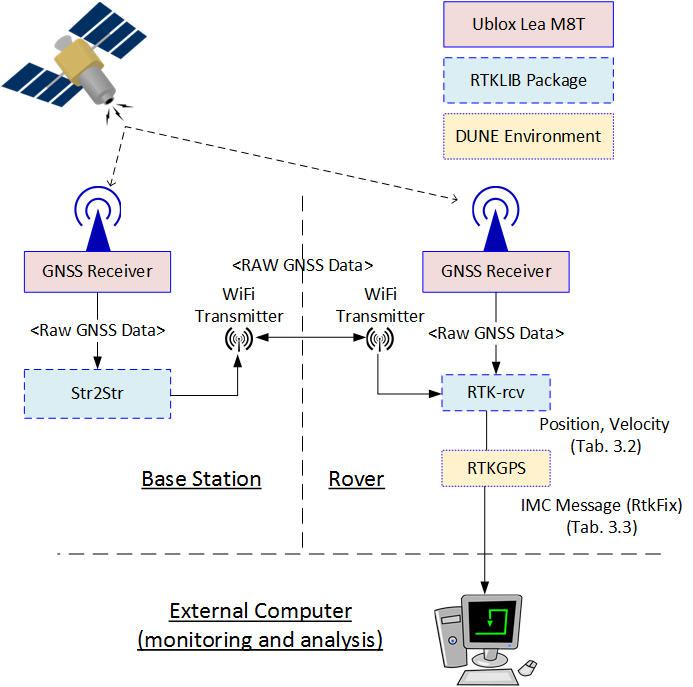
\includegraphics[width=1\textwidth]{figs/RTKLIB.png}
		\caption{The communication structure of \gls{rtklib}}
		\label{figure:RTKLIB_STRUCTURE}
\end{figure}
\subsubsection{Rtkrcv}
As part of the \gls{rtklib} Rtkrcv is  used to calculate the position of the rover in real time. Rtkrcv can be configured to have two output streams. It's desired in a automatic landing system to have a velocity estimate. However this is not provided in the newest version of \gls{rtklib}, and therefore a altered version of \gls{rtklib} is used in the navigation system where the velocity is part of the output data. The position output is in \gls{enu} format and the full output structure is presented in table \ref{Tb:RtklibOutput}
\begin{table}[H]
\begin{center}
    \begin{tabular}{ | l | l |}
    \hline
    \textbf{Header} & \textbf{Content} \\ \hline
     1 Time & The epoch time of the solution indicate the true receiver\\& signal reception time. Can have the following format:\\&\\& yyyy/mm/dd HH:MM:SS.SSS:\\& Calender time in GPST, UTC or JST.\\&\\&
     
     WWWW SSSSSSS.SSS:\\&
     GPS week and TOW in seconds  \\ \hline
     2 Receiver Position & The rover receive antenna position \\ \hline
     3 Quality flag (Q) & The flag which indicates the solution quality.\\& 1:Fixed\\& 2:Float\\& 5:Single \\ \hline
     4 Number of valid satellites (ns) & The number of valid satellites for solution estimation. \\ \hline
     5 Standard deviation & The estimated standard deviation of the\\& solution assuming a priori error model and error\\& parameters by the positioning options \\ \hline
     6 Age of differential & The time difference between the observation data epochs\\& of the rover receiver and base station in second. \\ \hline
     7 Ratio factor & The ratio factor of "ratio-test" for standard integer\\& ambiguity validation strategy \\ \hline
     8 Receiver velocity & The velocity of the rover. Given only when output is\\& in enu format \\ \hline
    \end{tabular}
\end{center}
\caption{Rtklib output solution format }
\label{Tb:RtklibOutput}
\end{table}
\subsubsection{Str2str}
Str2str is used as a base station program that can receive raw \gls{gnss} data and further export data over tcp, set-up by str2str. Str2str sends out Radio Technical Commission for Maritime Service 3 (RMTC3) formatted messages, however it can be configured to send whatever comes in as input. The communication between str2str and rtkrcv is shown i figure \ref{figure:RTKLIB_STRUCTURE}
\section{Pixhawk}
Pixhawk is a high-performance autopilot suitable for fixed wing multi rotors, helicopter and other robotic platform that can move. The Pixhawk system comes complete with \gls{gps}, imu, airspeed sensor and magnetometer.
\section{Ardupilot}
Ardupilot is an open-source unmanned aerial vehicle platform, able to control fixed wing \gls{uav} and multicopters. Ardupilot is used for low level control of the \gls{uav}, and is the software that runs on the Pixhawk. Ardupilot is able to communicate to third party software e.g Dune. Ardupilot uses the sensors in the Pixhawk to calculate the position, velocity and attitude of the \gls{uav}, which is sent to DUNE.
\section{JSBsim}
JSBSim \citep{berndt2004jsbsim} is an open-source flight dynamic model that is able to simulate a physical model of an arbitrary aircraft without the need of specific compiled and linked program code. The simulator is design such that a third party software e.g. Ardupilot can expose the model to external forces and moments. This enable SIL testing of system that is able to run in a hardware configuration with only minor configuration alteration.
\cleardoublepage